\documentclass[11pt,a4paper]{article}

\usepackage{pifont}
\usepackage{amsmath}
\usepackage{amssymb}
\usepackage{psfig}
\usepackage{graphicx}
\usepackage{array}
\usepackage{fancyheadings}
\usepackage{here}
\usepackage{eepic,epic}
\usepackage[english]{babel}

\input{YRpersdf}

\oddsidemargin -0.4cm
\evensidemargin -0.4cm
\topmargin -1cm
\textheight 22.5cm
\textwidth 16.6cm
\headheight 1.0cm

% principal notations



\begin{document}

\begin{center}
  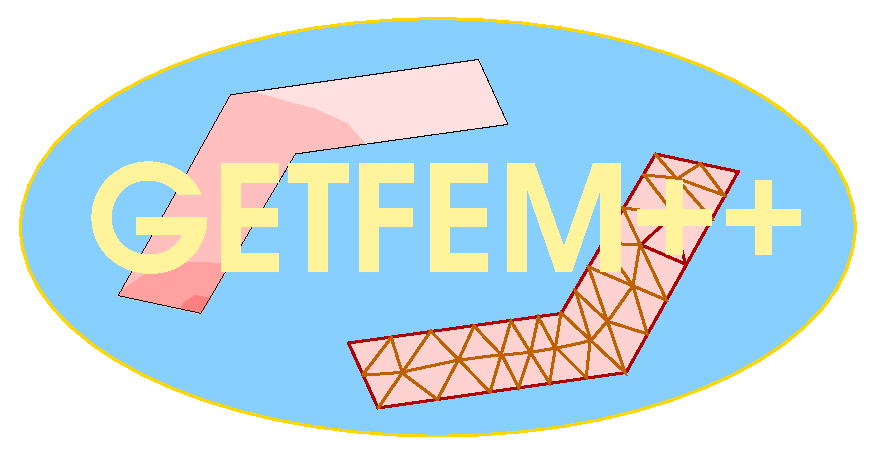
\includegraphics[width=10cm,angle=0]{getfem_logo.eps}\\[0.2cm]
  a Generic Finite Element library in C++ \\[0.5cm]
  \begin{largebox} \begin{center}
      \Huge \sc Description of Finite Element and Integration Methods
  \end{center}  \end{largebox}
  \\[0.5cm]
  { \large Yves \sc Renard\footnote{ \it MIP, INSAT, Complexe scientifique de Rangueil, 31077 Toulouse, France, Yves.Renard@gmm.insa-tlse.fr } } \\[1.0cm]
      July 31, 2002\\[1.0cm]
\end{center}

% \begin{abstract}
% Basic description of the structure of the finite element kernel of GETFEM++.
% \end{abstract}


%%%%%%%%%%%%%%%%%%%%%%%%%%%%%%%%%%%%%%%%%%%%%%%%%%%%%%%%%%%%%%%%%%%%%%%%%
%          INTRODUCTION                                                 %
%%%%%%%%%%%%%%%%%%%%%%%%%%%%%%%%%%%%%%%%%%%%%%%%%%%%%%%%%%%%%%%%%%%%%%%%%

\section*{Introduction}
This documentation describes the different finite element methods and approximative integration methods available in GETFEM++.\\[4cm]
Copyright (C) 2002\\
The program GETFEM++ is free software; you can redistribute it and/or modify
it under the terms of the GNU General Public License as published by
the Free Software Foundation; version 2 of the License.
This program is distributed in the hope that it will be useful,
but WITHOUT ANY WARRANTY; without even the implied warranty of
MERCHANTABILITY or FITNESS FOR A PARTICULAR PURPOSE.  See the
GNU General Public License for more details.
You should have received a copy of the GNU General Public License
along with this program; if not, write to the Free Software Foundation,
Inc., 59 Temple Place - Suite 330, Boston, MA  02111-1307, USA.

\newpage
\tableofcontents
\newpage

\section{Finite element methods}

\subsection{Finite element methods description}

A finite element method is defined on a reference element $\overline{T} \subset \Reel^P$ by a set of $n_d$ nodes $a^i$ and corresponding base functions 
$$ \overline{\varphi}^i : \overline{T} \subset \Reel^P \longrightarrow \Reel^Q, $$
Denoting
$$ \tilde{\varphi}^i(x) = \overline{\varphi}^i(\overline{x}) = \overline{\varphi}^i(\tau^{-1}(x)), $$
a linear transformation is allowed for the real base function
$$ \varphi^i(x) = \sum_{j = 0}^{n_d - 1} M_{ij} \tilde{\varphi}^j(x), $$
where $M$ is a $n_d \times n_d$ matrix possibly depending on the geometric transformation (i.e. on the real element).
We denote
$$ [\overline{\varphi}(\overline{x})] = \vecfour{\overline{\varphi}^0(\overline{x})}{\overline{\varphi}^1(\overline{x})}{...}{\overline{\varphi}^{n_d-1}(\overline{x})}, $$
the $n_d \times Q$ matrix, such that when a function is defined by
$$ f(x) = \sum_{i = 0}^{n_d - 1} \alpha_i \varphi^i(x), $$
one has
$$ \fbox{$\hspace{1em} f(\tau(\overline{x})) = \alpha^T M [\overline{\varphi}(\overline{x})],\hspace{1em}$} $$
where $\alpha$ is the vector of components $\alpha_i$.

A certain number of description of classical finite element method are defined in the file {\tt getfem\_fem.h}. More classical ones are the following:

\begin{center} \begin{tabular}{|m{0.55\linewidth}|m{0.4\linewidth}|} \hline
{\tt getfem::ppolyfem getfem::PK\_fem(n, k)} & Classical $P_K$ methods on simplexes of dimension  {\tt n} with degree {\tt k} polynomials.\\ \hline
{\tt getfem::ppolyfem getfem::QK\_fem(n, k)} & Classical $Q_K$ methods on parallelepiped of dimension {\tt n}. Tensorial product of degree {\tt k} $P_K$ method on the segment. \\ \hline
{\tt getfem::ppolyfem getfem::PK\_prism\_fem(n, k)} & Classical methods on prism of dimension {\tt n}. Tensorial product of two degree {\tt k} $P_K$ method. \\ \hline
{\tt getfem::ppolyfem getfem::product\_fem( ppolyfem\;a, ppolyfem b)} & Tensorial product of the two polynomial finite element method {\tt a} and {\tt b}. \\ \hline
{\tt getfem::ppolyfem $\;$ getfem::P1\_nonconforming\_fem()} & Non conforming $P_1$ method on triangles. \\ \hline
\end{tabular} \end{center}


One can see in the file {\tt getfem\_fem.C} how to define a new finite element method. Basically, the only thing to do is to give the base functions on the reference element and the corresponding nodes.

\subsubsection{graphical codification of d.o.f.}

\begin{figure}[H] \label{fig:symbols}
  \begin{center}
    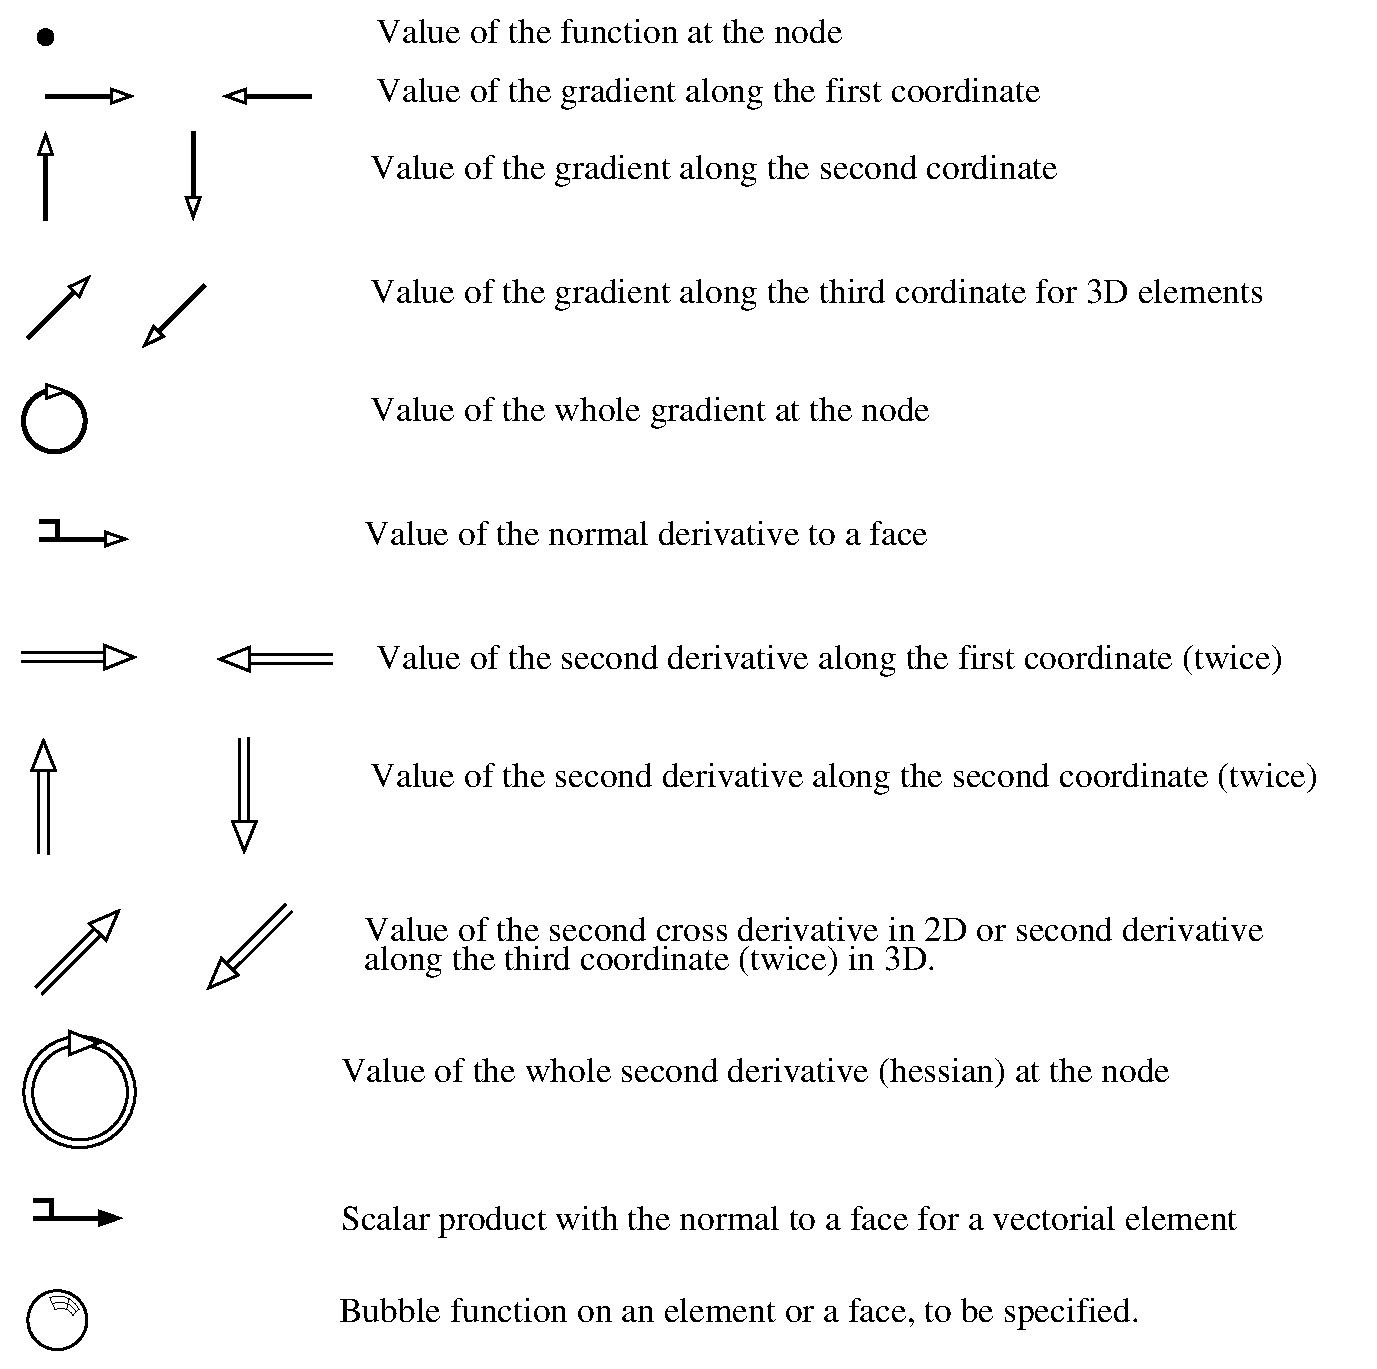
\includegraphics[width=13cm,angle=0]{getfemlist_symbols.eps}
  \end{center}
  \caption{ \it Symbols representing degree of freedom types}
\end{figure}

\subsection{Basic Lagrange elements on simplexes}

a chaque �l�ment : 
dessin des ddl avec code
nb de ddl, degre, equivalence via la transformation g�ometrique, vectoriel ou non, analyse du raccord

\subsection{Basic Lagrange elements on other geometries}

\begin{figure}[H] \label{fig:symbols}
  \begin{center}
    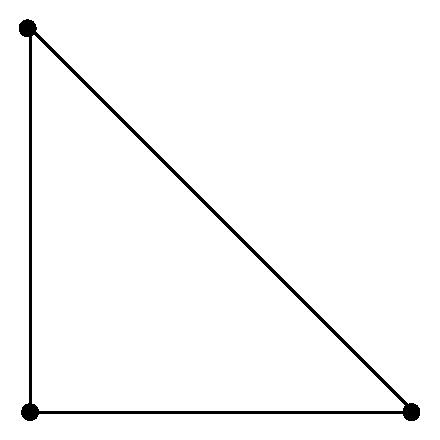
\includegraphics[width=5cm,angle=0]{getfemlist_triangle_P1.eps}
  \end{center}
  \caption{ \it$P_1$ standard Lagrange element on a triangle, 3 d.o.f., $C^0$}
\end{figure}

\begin{figure}[H] \label{fig:symbols}
  \begin{center}
    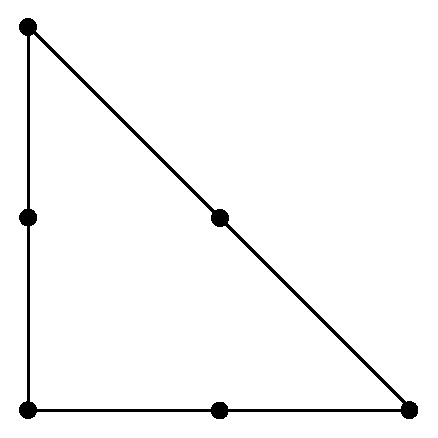
\includegraphics[width=5cm,angle=0]{getfemlist_triangle_P2.eps}
  \end{center}
  \caption{ \it$P_2$ standard Lagrange element on a triangle, 6 d.o.f., $C^0$}
\end{figure}

\begin{figure}[H] \label{fig:symbols}
  \begin{center}
    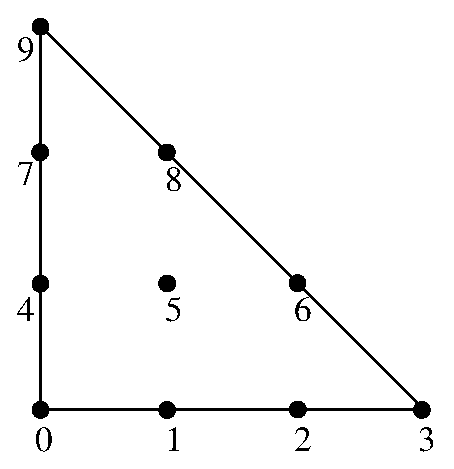
\includegraphics[width=5cm,angle=0]{getfemlist_triangle_P3.eps}
  \end{center}
  \caption{ \it$P_3$ standard Lagrange element on a triangle, 10 d.o.f., $C^0$}
\end{figure}

\begin{figure}[H] \label{fig:symbols}
  \begin{center}
    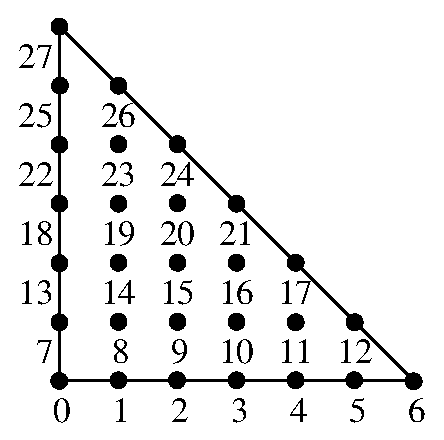
\includegraphics[width=5cm,angle=0]{getfemlist_triangle_P6.eps}
  \end{center}
  \caption{ \it$P_6$ standard Lagrange element on a triangle, 28 d.o.f., $C^0$}
\end{figure}

\begin{figure}[H] \label{fig:symbols}
  \begin{center}
    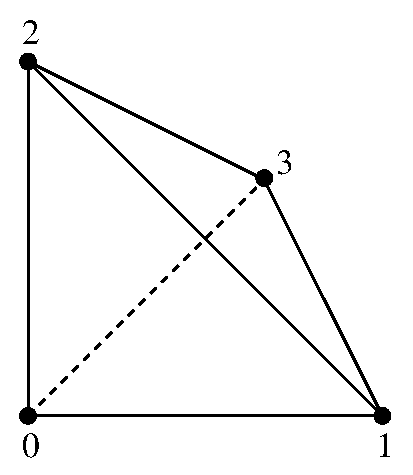
\includegraphics[width=5cm,angle=0]{getfemlist_tetrahedron_P1.eps}
  \end{center}
  \caption{ \it$P_1$ standard Lagrange element on a tetrahedron, 4 d.o.f., $C^0$}
\end{figure}

\begin{figure}[H] \label{fig:symbols}
  \begin{center}
    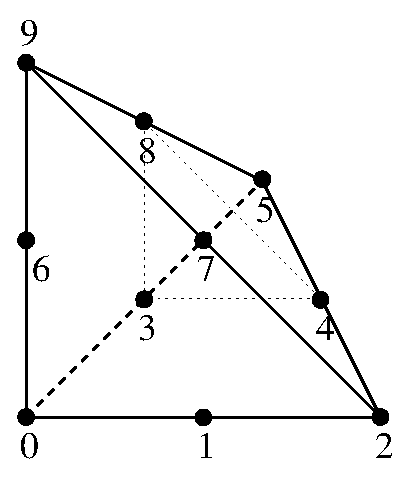
\includegraphics[width=5cm,angle=0]{getfemlist_tetrahedron_P2.eps}
  \end{center}
  \caption{ \it$P_2$ standard Lagrange element on a tetrahedron, 10 d.o.f., $C^0$}
\end{figure}


\subsection{Specific elements in dimension 1}


\subsection{Specific elements in dimension 2}


\begin{figure}[H] \label{fig:symbols}
  \begin{center}
    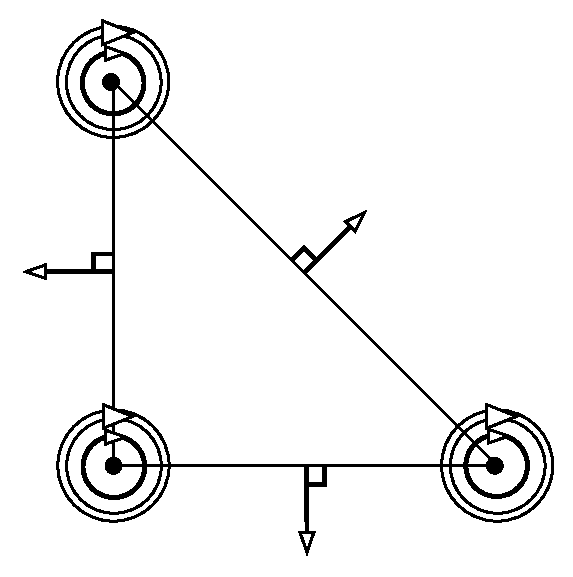
\includegraphics[width=6cm,angle=0]{getfemlist_argyris.eps}
  \end{center}
  \caption{ \it Argyris element, $P_5$, 21 d.o.f., $C^1$}
\end{figure}

\subsection{Specific elements in dimension 3}


\subsection{Tensorial product of elements}


\section{Integration methods}

\subsection{Integration methods description}

The integrations methods are of two kinds. The file {\tt bgeot\_poly\_integration.h} defines exact integrations of polynomials and the file {\tt bgeot\_approx\_integration.h} defines approximated integrations of any function. The exact integration can only be used if all the elements are polynomial and if the geometric transformation is linear.

In the file {\tt bgeot\_poly\_integration.h} the following functions are defined

\begin{center} \begin{tabular}{|m{0.55\linewidth}|m{0.4\linewidth}|} \hline
{\tt "IM\_EXACT\_SIMPLEX(n)"} & Description of the exact integration of polynomials on the simplex of reference of dimension {\tt n}. \\ \hline
\end{tabular}  
\begin{tabular}{|m{0.55\linewidth}|m{0.4\linewidth}|} \hline
{\tt "IM\_PRODUCT(a, b)"} & Description of the exact integration on the convex which is the direct product of the convex in {\tt a} and in {\tt b}.\\ \hline
\end{tabular}  
\begin{tabular}{|m{0.55\linewidth}|m{0.4\linewidth}|} \hline
{\tt "IM\_EXACT\_PARALLELEPIPED(n)"} & Description of the exact integration of polynomials on the parallelepiped of reference of dimension {\tt n}\\ \hline
\end{tabular}  
\begin{tabular}{|m{0.55\linewidth}|m{0.4\linewidth}|} \hline
{\tt "IM\_EXACT\_PRISM(n)"} & Description of the exact integration of polynomials on the prism of reference of dimension {\tt n}\\ \hline
\end{tabular} \end{center}


Even though a description of exact integration method exists on parallelepipeds or prisms, most of the time the geometric transformations on such elements are not linear and the exact integration cannot be used.

In the file {\tt bgeot\_approx\_integration.h} the following functions are defined

\begin{center} \begin{tabular}{|m{0.55\linewidth}|m{0.4\linewidth}|} \hline
{\tt "IM\_GAUSS1D(k)" } & Description of the Gauss integration on a segment of order {\tt k}. \\ \hline
\end{tabular}  
\begin{tabular}{|m{0.55\linewidth}|m{0.4\linewidth}|} \hline
{\tt "IM\_NC(n,k)"} & Description of the integration on a simplex of reference of dimension {\tt n} for polynomials of degree {\tt k} with the Newton Cotes method (based on Lagrange interpolation).\\ \hline
\end{tabular}  
\begin{tabular}{|m{0.55\linewidth}|m{0.4\linewidth}|} \hline
{\tt "IM\_PRODUCT(a,b)"} & Build a method doing the direct product of methods {\tt a} and {\tt b}. \\ \hline
\end{tabular}  
\begin{tabular}{|m{0.55\linewidth}|m{0.4\linewidth}|} \hline
{\tt "IM\_TRIANGLE(2)"} & Integration on a triangle of order 2 with 3 points. \\ \hline
\end{tabular}
\begin{tabular}{|m{0.55\linewidth}|m{0.4\linewidth}|} \hline
{\tt "IM\_TRIANGLE(7)"} & Integration on a triangle of order 7 with 13 points. \\ \hline
\end{tabular} 
\begin{tabular}{|m{0.55\linewidth}|m{0.4\linewidth}|} \hline
{\tt "IM\_QUAD(2)"} & Integration on quadrilaterals of order 2 with 3 points. \\ \hline
\end{tabular}
\begin{tabular}{|m{0.55\linewidth}|m{0.4\linewidth}|} \hline
{\tt "IM\_TETRAHEDRON(5)"} & Integration on a tetrahedron of order 5 with 15 points. \\ \hline
\end{tabular} \end{center}


Other methods can be easily defined.

\subsection{Exact Integration methods}

\subsection{Newton cotes Integration methods}

\subsection{Gauss Integration methods on dimension 1}

\subsection{Gauss Integration methods on dimension 2}

\subsection{Gauss Integration methods on dimension 3}

\subsection{Direct product of integration methods}


\begin{thebibliography}{99}
% \bibliographystyle{apalike}
% \bibliographystyle{plain}
% \bibliography{all}
\bibitem{dh-to1984} 
  G. {\sc Dhatt, and  G. Touzot}
  {\it The Finite Element Method Displayed}, 
 J. Wiley \& Sons,  New York, 1984.

\bibitem{BAS_COMP}
  Y. {\sc Renard},
  {\it Elementary Computations in GETFEM++}, 2002.

\bibitem{USER_DOC}
  Y. {\sc Renard},
  {\it Short User Documentation of GETFEM++}, 2002.

\bibitem{nedelec1991}
  J.-C. {\sc Nedelec},
  {\it Notions sur les techniques d'�l�ments finis}, Ellipses, SMAI, Math�matiques \& Applications n�7, 1991.
\end{thebibliography}


\end{document}
